\def \kaflanr {11}
\lecture[\kaflanr]{\kaflanr. Lagrange-margfaldarar}{lecture-text}
\date{9.~febrúar 2015}
\newcounter{mycount}
\refstepcounter{mycount}

\begin{document}

\begin{frame}
	\maketitle
\end{frame}




\begin{frame}{Útgildi falla þar sem breytur uppfylla skorðujöfnur} 

\begin {block}{Sértækar aðferðir \kaflanr.\arabic{mycount}}\stepcounter{mycount}
Finna skal útgildi falls $f(x,y)$ þegar skilgreiningarsvæði $f$ er mengi þeirra punkta $(x,y)$ sem uppfylla jöfnu $g(x,y)=0$.  


\begin {enumerate}
 \item Er mögulegt að einangra $x$ eða $y$ í jöfnunni $g(x,y)=0$?  
 
 \medskip
 \begin {itemize}
  \item [] Ef hægt er að einangra $y$ og rita $y=h(x)$ þá snýst verkefnið nú um að finna útgildi falls $f(x,h(x))$ af einni breytu $x$.

 \end {itemize}
 \item  Er hægt að stika ferilinn $g(x,y)=0$?  
 
 \begin {itemize}
  \item [] Ef $\rv$ er stikun á
     ferlinum þá þurfum við að leita að útgildum fallsins $f(\rv(t))$ þar sem
     er bara ein breyta.  
 \end {itemize}

\end {enumerate}

\end{block}

\end{frame}




\begin {frame}{Dæmi}
 \begin {figure}[h!]
 \centering
            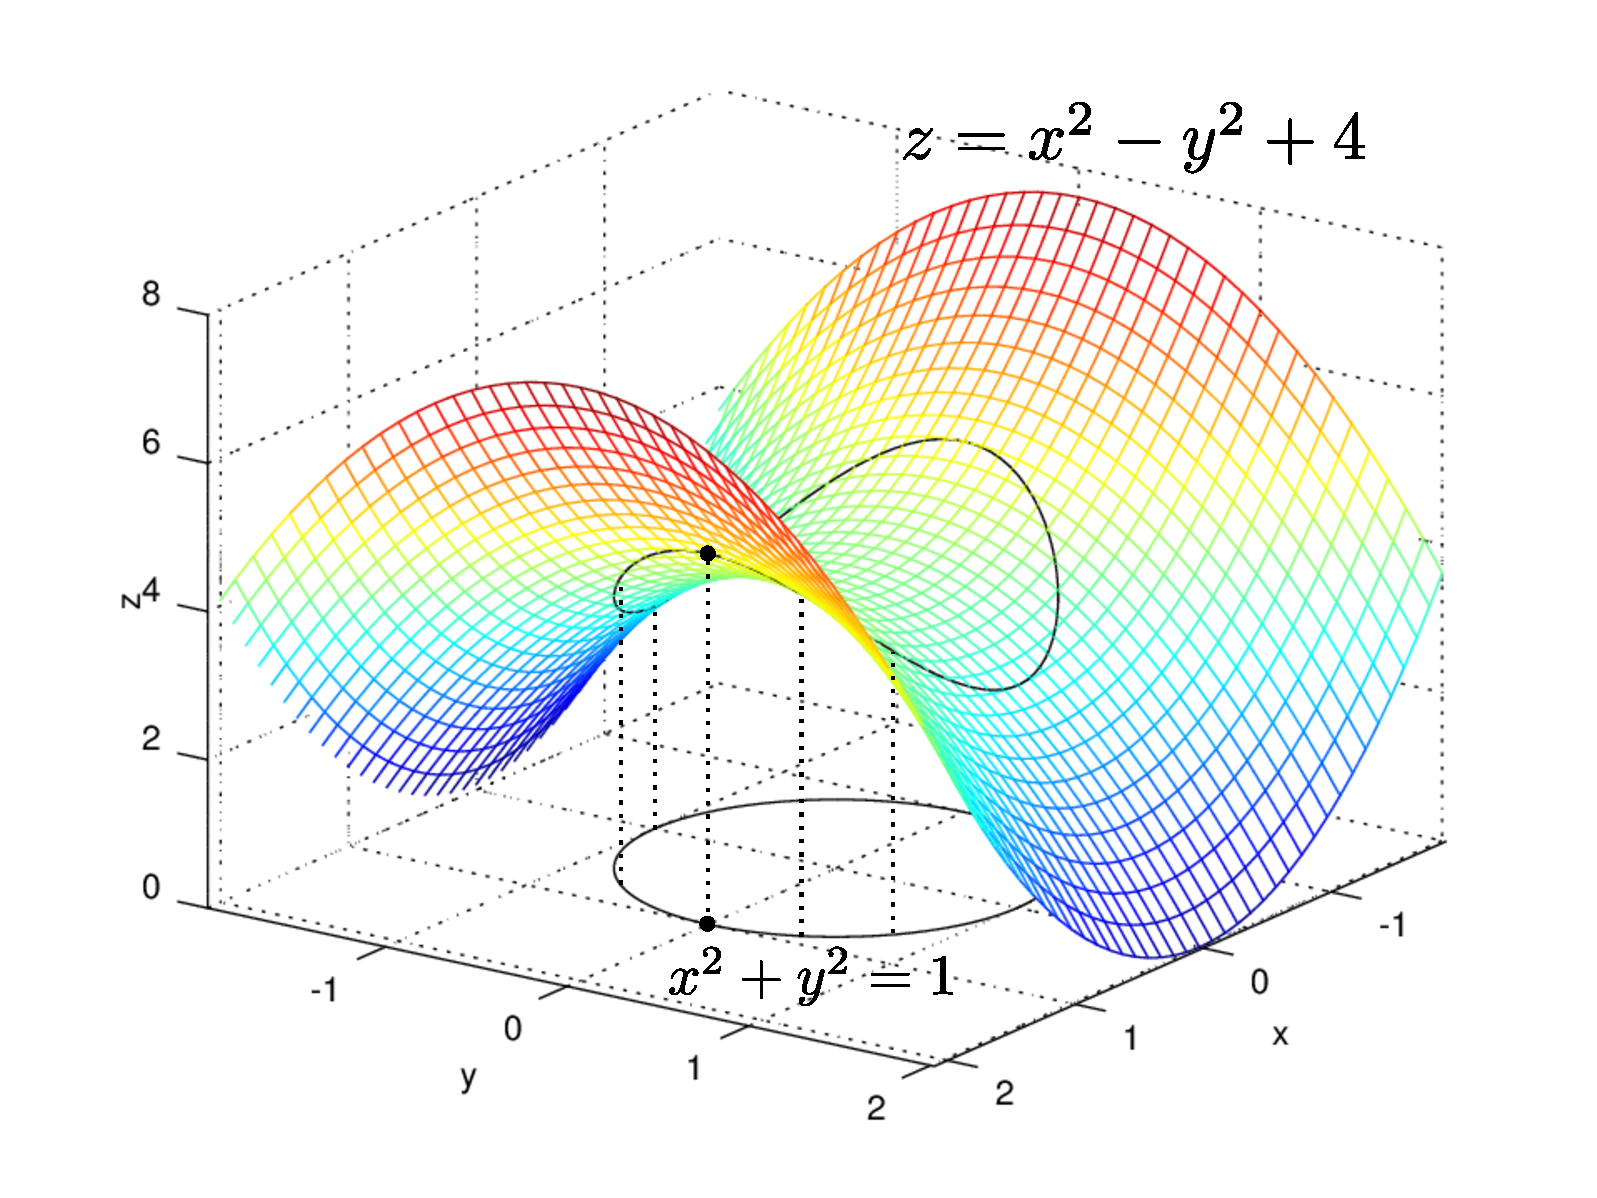
\includegraphics[width=.7\linewidth]{constraint.pdf}
            \caption*{Hver eru hæstu og lægstu gildi fallsins $f(x,y) = x^2-y^2+4$ á menginu $\{(x,y)~|~x^2+y^2=1\}$?}
\end {figure}
\end {frame}



 


\begin{frame}{Útgildi falla þar sem breytur uppfylla skorðujöfnur} 

\begin {block}{Setning \kaflanr.\arabic{mycount}}\stepcounter{mycount}
Látum $f$ og $g$ vera föll sem eru bæði
diffranleg í punktinum $P_0=(x_0,y_0)$ sem liggur á ferlinum
$g(x,y)=0$, og er ekki endapunktur ferilsins.  Gerum ráð fyrir að
$\nabla g(x_0,y_0)\neq \ov$.  Gerum líka ráð fyrir að ef við einskorðum fallið $f$ við ferilinn $g(x,y)=0$ þá hafi $f$ staðbundið útgildi í $P_0$.  Þá eru stiglarnir $\nabla f(x_0,y_0)$ og $\nabla g(x_0,y_0)$ samsíða.
\end{block}
\end {frame}
\begin {frame}
\begin {figure}[h!]
 \centering
            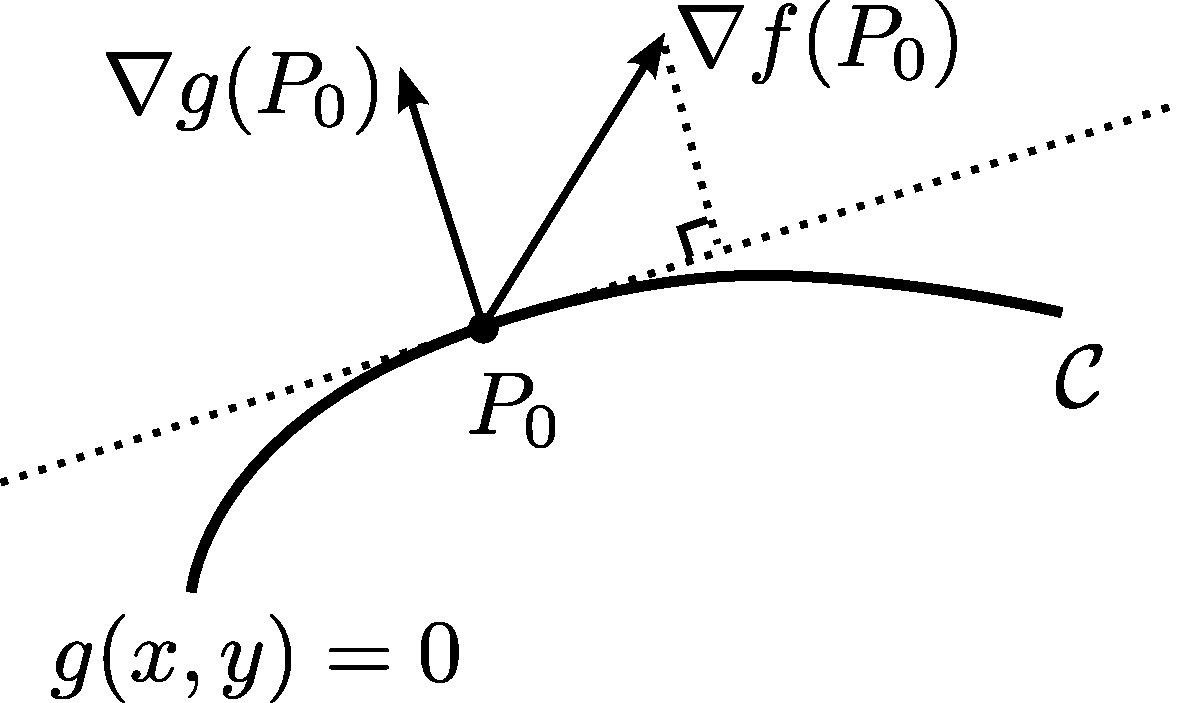
\includegraphics[width=.4\linewidth]{lagrange1}
            \caption*{Ef stiglarnir $\nabla g(P_0)$ og $\nabla f(P_0)$ eru ekki samsíða þá vex $f$ eða minnkar þegar farið er eftir $\mathcal{C}$ út frá punktinum $P_0$.}
\end {figure}
\end{frame}


\begin{frame}{Lagrange-margfaldarar} 

\begin {block}{Reikniaðferð \kaflanr.\arabic{mycount}}\stepcounter{mycount}
  Finna skal útgildi falls $f(x,y)$ þegar skilgreiningarsvæði $f$ er mengi þeirra punkta $(x,y)$ sem uppfylla jöfnu $g(x,y)=0$.  

\medskip
Búum til {\em Lagrange-fallið}
$$L(x,y,\lambda)=f(x,y)+\lambda g(x,y).$$
Stöðupunktar $L$, þ.e.a.s.~punktar $(x_0,y_0,\lambda_0)$ þar sem $\nabla L(x_0,y_0,\lambda_0)=\ov$, gefa mögulega punkta $(x_0,y_0)$ þar sem $f$ tekur útgildi.

\medskip
Þessir punktar finnast með því að leysa jöfnuhneppið
\begin{align*}
f_1(x,y)+\lambda g_1(x,y)&=0\\
f_2(x,y)+\lambda g_2(x,y)&=0\\
g(x,y)&=0.
\end{align*}
\end{block}
Talan $\lambda$ nefnist \emph{Lagrange-margfaldari}.
\end{frame}


\begin{frame}{Lagrange-margfaldarar} 

\begin {block}{Regla \kaflanr.\arabic{mycount}}\stepcounter{mycount}
Finna skal útgildi falls $f(x,y)$ þegar skilgreiningarsvæði $f$ er mengi þeirra punkta $(x,y)$ sem uppfylla jöfnu $g(x,y)=0$.  

Athuga þarf punkta sem uppfylla eitt af eftirfarandi skilyrðum:

\begin {enumerate}
 \item Stöðupunktar $L(x,y,\lambda)$.
\item Punktar $(x,y)$ þar sem $\nabla g(x,y)=\ov$.
\item  Punktar $(x,y)$ þar sem annar eða báðir stiglanna $\nabla
      g(x,y)$ og $\nabla f(x,y)$ eru ekki skilgreindir. 
\item ,,Endapunktar\lq\lq\ ferilsins $g(x,y)=0$.
 \end {enumerate}

\end{block}

\end{frame}


\begin{frame}{} 

\begin {block}{Reikniaðferð \kaflanr.\arabic{mycount}}\stepcounter{mycount}
Finna skal útgildi falls $f(x,y,z)$ þegar skilgreiningarsvæði $f$ er mengi þeirra punkta $(x,y,z)$ sem uppfylla jöfnurnar $g(x,y,z)=0$ og $h(x,y,z)=0$.  

Búum til Lagrange-fallið
$$L(x,y,z,\lambda,\mu)=f(x,y,z)+\lambda g(x,y,z)+\mu h(x,y,z).$$
Stöðupunktar $L$, þ.e.a.s.~punktar $(x_0,y_0,z_0,\lambda_0,\mu_0)$ þar sem $\nabla L(x_0,y_0,z_0,\lambda_0,\mu_0)=\ov$ gefa mögulega punkta $(x_0,y_0,z_0)$ þar sem $f$ tekur útgildi.

Þessir punktar finnast með því að leysa jöfnuhneppið
\begin{align*}
f_1(x,y,z)+\lambda g_1(x,y,z)+\mu h_1(x,y,z)&=0\\
f_2(x,y,z)+\lambda g_2(x,y,z)+\mu h_2(x,y,z)&=0\\
f_3(x,y,z)+\lambda g_3(x,y,z)+\mu h_3(x,y,z)&=0\\
g(x,y,z)&=0\\
h(x,y,z)&=0.
\end{align*}
\end{block}

\end{frame}




\end{document}